\documentclass[tikz, convert={outfile=\jobname.png}]{standalone}
\input{../../tikzpic_packages.tex}

\begin{document}
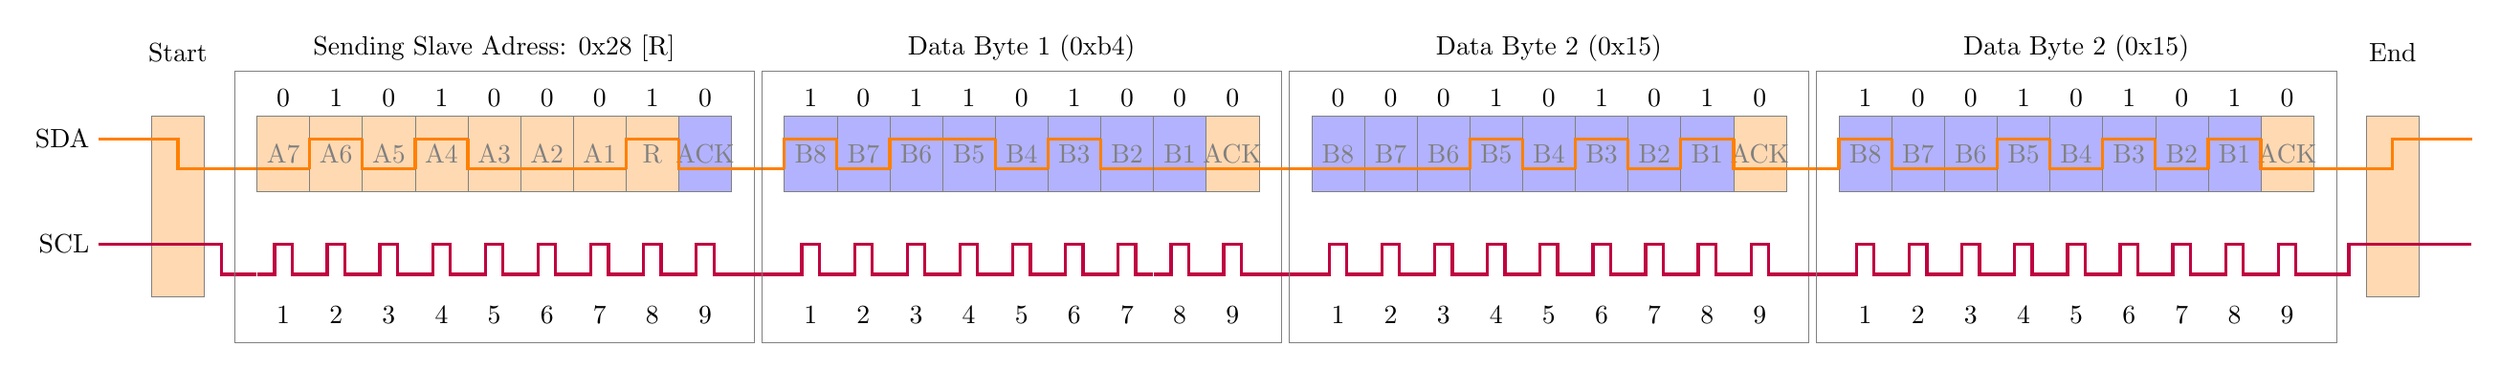
\begin{tikzpicture}[
scale = 1,
arrow/.style={-latex},
sda/.style={orange, very thick},
scl/.style={purple, very thick},
note/.style={help lines},
master/.style={fill=orange!30},
slave/.style={fill=blue!30}
]

\def\sdah{2.4}
\def\sdal{2}
\pgfmathsetmacro{\sdastep}{\sdah-\sdal}
\def\sclh{1}
\def\scll{.6}
\pgfmathsetmacro{\sclstep}{\sclh-\scll}


\def\frameb{.3}
\def\step{.7}
\pgfmathsetmacro{\steph}{\step*.5}
\pgfmathsetmacro{\stepd}{\step*.333}


%% Functions
\newcommand{\startseq}[1]{
\draw[note, master] (#1+\step,\sdah+\frameb)rectangle(#1+\step+\step,\scll-\frameb);
\draw[sda] (#1,\sdah)--++(\step,0)--++(\steph,0)--++(0,-\sdastep)--++(\steph,0)--++(\step,0);
\draw[scl] (#1,\sclh)--++(\step,0)--++(\step,0)--++(\stepd,0)--++(0,-\sclstep)--++(\stepd,0)--++(\stepd,0);
\path (#1+\step+\steph,\sdah+\frameb+.6)node[above]{Start};
}
\newcommand{\finalseq}[1]{
\draw[note, master] (#1+\step,\sdah+\frameb)rectangle(#1+\step+\step,\scll-\frameb);
\draw[sda] (#1,\sdal)--++(\step,0)--++(\steph,0)--++(0,\sdastep)--++(\steph,0)--++(\step,0);
\draw[scl] (#1,\scll)--++(\stepd,0)--++(\stepd,0)--++(0,\sclstep)--++(\stepd,0)--++(\step,0)--++(\step,0);
\path (#1+\step+\steph,\sdah+\frameb+.6)node[above]{End};
}
\newcommand{\datatransfer}[2]{
\ifnum #2=1 \def\level{\sdah} \fi
\ifnum #2=0 \def\level{\sdal} \fi
\ifnum \lastbit=1 \def\lastlevel{\sdah} \fi
\ifnum \lastbit=0 \def\lastlevel{2} \fi
\draw[sda] (#1,\lastlevel)--(#1,\level)--++(\step,0);
\draw[scl] (#1,\scll)--++(\stepd,0)--++(0,\sclstep)--++(\stepd,0)--++(0,-\sclstep)--++(\stepd,0);
\pgfmathparse{\lastx +\step}
\global\let\lastx\pgfmathresult
\global\let\lastbit\bit
}
\newcommand{\pausesignal}[1]{
\ifnum \lastbit=1 \def\lastlevel{\sdah} \fi
\ifnum \lastbit=0 \def\lastlevel{2} \fi
\draw[sda] (#1,\lastlevel)--(#1,\lastlevel)--++(\step,0);
\draw[scl] (#1,\scll)--++(\step,0);
\pgfmathparse{\lastx +\step}
\global\let\lastx\pgfmathresult
}


%% Signal

%% Start Seq
\path (0,\sdah)node[left]{SDA};
\path (0,\sclh)node[left]{SCL};
\startseq{0}

%% Write Slave Adress
\pgfmathsetmacro{\lastx}{3*\step}
\pgfmathsetmacro{\startx}{\lastx}
\def\lastbit{0}
\foreach[count=\i] \bit in {0,1,0,1,0,0,0,1,0}{
	% Notes
	\pgfmathtruncatemacro{\j}{8-\i}
	\def\text{A\j}
	\def\fillcol{master}
	\ifnum\i=8 \def\text{R} \fi
	\ifnum\i=9 \def\text{ACK} \def\fillcol{slave} \fi	
	\draw[note, \fillcol] (\lastx,\sdah+\frameb)rectangle(\lastx+\step,\sdal-\frameb)node[midway]{\text};
	\path (\lastx+\steph,\sdah+\frameb)node[above]{\bit};
	\path (\lastx+\steph,\scll-\frameb)node[below]{\i};
	% Draw the line
	\datatransfer{\lastx}{\bit}
}
\draw[note] (\startx-\frameb,\sdah+\frameb+.6)rectangle(\lastx+\frameb,\scll-\frameb-.6);
\path (\startx-\frameb,\sdah+\frameb+.6)--(\lastx+\frameb,\sdah+\frameb+.6)node[midway, above]{
	Sending Slave Adress: 0x28 [R]};


%% One Step Pause
\pausesignal{\lastx}


%% Read from Slave
\pgfmathsetmacro{\startx}{\lastx}
\foreach[count=\i] \bit in {1,0,1,1,0,1,0,0,0}{
	% Notes
	\pgfmathtruncatemacro{\j}{9-\i}
	\def\text{B\j}
	\def\fillcol{slave}
	\ifnum\i=9 \def\text{ACK} \def\fillcol{master} \fi	
	\draw[note, \fillcol] (\lastx,\sdah+\frameb)rectangle(\lastx+\step,\sdal-\frameb)node[midway]{\text};
	\path (\lastx+\steph,\sdah+\frameb)node[above]{\bit};
	\path (\lastx+\steph,\scll-\frameb)node[below]{\i};
	% Draw the line
	\datatransfer{\lastx}{\bit}
}
\draw[note] (\startx-\frameb,\sdah+\frameb+.6)rectangle(\lastx+\frameb,\scll-\frameb-.6);
\path (\startx-\frameb,\sdah+\frameb+.6)--(\lastx+\frameb,\sdah+\frameb+.6)node[midway, above]{
	Data Byte 1 (0xb4)};

%% One Step Pause
\pausesignal{\lastx}

%% Read from Slave
\pgfmathsetmacro{\startx}{\lastx}
\foreach[count=\i] \bit in {0,0,0,1,0,1,0,1,0}{
	% Notes
	\pgfmathtruncatemacro{\j}{9-\i}
	\def\text{B\j}
	\def\fillcol{slave}
	\ifnum\i=9 \def\text{ACK} \def\fillcol{master} \fi	
	\draw[note, \fillcol] (\lastx,\sdah+\frameb)rectangle(\lastx+\step,\sdal-\frameb)node[midway]{\text};
	\path (\lastx+\steph,\sdah+\frameb)node[above]{\bit};
	\path (\lastx+\steph,\scll-\frameb)node[below]{\i};
	% Draw the line
	\datatransfer{\lastx}{\bit}
}
\draw[note] (\startx-\frameb,\sdah+\frameb+.6)rectangle(\lastx+\frameb,\scll-\frameb-.6);
\path (\startx-\frameb,\sdah+\frameb+.6)--(\lastx+\frameb,\sdah+\frameb+.6)node[midway, above]{
	Data Byte 2 (0x15)};


%% One Step Pause
\pausesignal{\lastx}

%% Read from Slave
\pgfmathsetmacro{\startx}{\lastx}
\foreach[count=\i] \bit in {1,0,0,1,0,1,0,1,0}{
	% Notes
	\pgfmathtruncatemacro{\j}{9-\i}
	\def\text{B\j}
	\def\fillcol{slave}
	\ifnum\i=9 \def\text{ACK} \def\fillcol{master} \fi	
	\draw[note, \fillcol] (\lastx,\sdah+\frameb)rectangle(\lastx+\step,\sdal-\frameb)node[midway]{\text};
	\path (\lastx+\steph,\sdah+\frameb)node[above]{\bit};
	\path (\lastx+\steph,\scll-\frameb)node[below]{\i};
	% Draw the line
	\datatransfer{\lastx}{\bit}
}
\draw[note] (\startx-\frameb,\sdah+\frameb+.6)rectangle(\lastx+\frameb,\scll-\frameb-.6);
\path (\startx-\frameb,\sdah+\frameb+.6)--(\lastx+\frameb,\sdah+\frameb+.6)node[midway, above]{
	Data Byte 2 (0x15)};


%% Ende
\finalseq{\lastx}




\end{tikzpicture}
\end{document}